\documentclass[a4paper]{article}

\usepackage{fullpage} % Package to use full page
\usepackage{parskip} % Package to tweak paragraph skipping
\usepackage{tikz} % Package for drawing
\usepackage{amsmath}
\usepackage{hyperref}
\usepackage{ctex}
\usepackage{listings}
\usepackage{diagbox}

%导言区的此三行无变化
\usepackage{graphicx}
\usepackage{float} 
\usepackage{subfigure}
\usepackage{caption}
\usepackage{tabularx}
\DeclareMathOperator*{\argmax}{argmax} 
\DeclareMathOperator*{\argmin}{argmin}

\renewcommand\thefigure{\thesection.\arabic{figure}}
\makeatletter
\@addtoreset{figure}{section}
\makeatother

\renewcommand\thetable{\thesection.\arabic{table}}
\makeatletter
\@addtoreset{table}{section}
\makeatother

\makeatletter
\renewcommand \theequation {%
	\ifnum \c@section>\z@ \@arabic\c@section.\fi \ifnum \c@subsection>\z@
	\@arabic\c@subsection.\fi\ifnum \c@subsubsection>\z@
	\@arabic\c@subsubsection.\fi\@arabic\c@equation}
\@addtoreset{equation}{section}
\@addtoreset{equation}{subsection}
%\setcounter{section}{-1}
\makeatother
%\captionsetup[figure]{labelfont={bf},name={Fig.},labelsep=period}
%\captionsetup[table]{labelfont={bf},name={Table.},labelsep=period}
\setlength{\parindent}{2em}

\lstset{
	columns=fixed,       
	numbers=left,                                        % 在左侧显示行号
	numberstyle=\tiny\color{gray},                       % 设定行号格式
	frame=none,                                          % 不显示背景边框
	backgroundcolor=\color[RGB]{245,245,244},            % 设定背景颜色
	keywordstyle=\color[RGB]{40,40,255},                 % 设定关键字颜色
	numberstyle=\footnotesize\color{darkgray},           
	commentstyle=\it\color[RGB]{0,96,96},                % 设置代码注释的格式
	stringstyle=\rmfamily\slshape\color[RGB]{128,0,0},   % 设置字符串格式
	showstringspaces=false,                              % 不显示字符串中的空格
	language=c++,                                        % 设置语言
}

\usepackage{algorithm}
\usepackage{algorithmicx}
\usepackage{algpseudocode}
\floatname{algorithm}{算法}
\renewcommand{\algorithmicrequire}{\textbf{输入:}}  
\renewcommand{\algorithmicensure}{\textbf{输出:}} 


\begin{document}

%\maketitle
\newcommand{\HRule}{\rule{\linewidth}{0.5mm}}
\begin{titlepage}
	\begin{center}
		% Upper part of the page
		
\includegraphics[width=0.4\textwidth]{Tsinghua2.png}\\[1cm]
		\textsc{\Large \texttt{多媒体通信技术}}\\[1cm]
		% Title
		\HRule \\[1cm]
		{\Huge \bfseries 基于聚类的图像分割算法}\\[0.4cm]
		\HRule \\[3.5cm]
		% Author and supervisor
		\begin{minipage}{0.4\textwidth}
			\begin{center}
				\Large
				\begin{tabular}{cc}
					\texttt{作者:} & 罗雁天 \\[0.5cm]
					\texttt{学号:} & 2018310742 \\[0.5cm]
					\texttt{日期:} & \today
				\end{tabular}
			\end{center}
		\end{minipage}
		\vfill
	\end{center}
\end{titlepage}


\tableofcontents
\newpage

\section{问题描述}
在计算机视觉领域,图像分割 (Segmentation) 指的是将 数字图像细分为多个图像子区域 (像素的集合)(也被称作超像 素) 的过程。图像分割的目的是简化或改变图像的表示形式, 使得图像更容易理解和分析。图像分割通常用于定位图像中 的物体和边界 (线,曲线等)。更精确的,图像分割是对图像 中的每个像素加标签的一个过程,这一过程使得具有相同标 签的像素具有某种共同视觉特性。

简单来说,图像分割可以看做是像素级别的分类,其在 医疗领域、自动驾驶等方面有着重要的应用,在目前的算法 研究中,图像分类可以分为Semantic Segmentation(语义分割)和 Instance Segmentation(实例分割)。

本次大作业采用首先采用传统机器学习中聚类的方式来进行图像的语义分割,然后使用近几年较好的算法与其进行对比。

\section{算法描述}
在本节首先介绍传统机器学习中的聚类算法,然后介绍一种基于条件随机场与循环神经网络的算法。

\subsection{Kmeans聚类算法}
聚类算法是一种无监督学习的算法,训练样本的标记信息是未知的,目标通过对无标记训练样本的学习来揭示数据的内在性质及规律,为进一步的数据分析提供基础。基于聚类的图像分割不需要很大的训练集来进行监督训练,相比于当前基于深度学习的图像分割算法训练时间更短。

给定样本集$D=\{x_1,x_2,\cdots,x_m \}$,“k均值”(kmeans)算法针对聚类所得簇划分$\mathcal{C}=\{C_1,C_2,\cdots\\,C_k \}$最小化平方误差:
\begin{equation}
\label{eq1}
E=\sum_{i=1}^{k}\sum_{x\in C_i}||x-\mu_i||_2^2
\end{equation}
其中,$\mu_i=\frac{1}{|C_i|}\sum_{x\in C_i}x$是簇$C_i$的均值向量。直观来看,式(\ref{eq1})在一定程度上刻画了簇内样本围绕簇均值向量的紧密程度,$E$值越小则簇内样本相似度越高。

KMeans算法流程如算法\ref{alg:kmeans}所示,其中第1行对均值向量进行初始化,在第4-8行与第9-16行依次对当前簇划分及均值向量迭代更新,若迭代更新后聚类结果保持不变,则将当前簇划分结果返回。

\begin{algorithm}[htbp]
	\caption{KMeans聚类算法}
	\label{alg:kmeans}
	\begin{algorithmic}[1]
		\Require 样本集$D=\{x_1,x_2,\cdots,x_m \}$,聚类簇数$k$
		\Ensure 簇划分$\mathcal{C}=\{C_1,C_2,\cdots,C_k \}$
		\State 从$D$中随机选择$k$个样本作为初始均值向量$\{\mu_1,\mu_2,\cdots,\mu_k \}$
		\Repeat 
		\State 令$C_i=\emptyset(1\le i\le k)$
		\For {$j=1,2,\cdots,m$}
		\State 计算样本$x_j$与各均值向量$\mu_i(1\le i\le k)$的距离:$d_{ji}=||x_j-x_i||_2^2$;
		\State 根据距离最近的均值向量确定$x_j$的簇标记:$\lambda_j=\argmin_{i\in {1,2,\cdots,k}}d_{ji}$;
		\State 将样本$x_j$划入相应的簇:$C_{\lambda_j}=C_{\lambda_j}\cup\{x_j\}$;
		\EndFor
		\For {$i=1,2,\cdots,k$}
		\State 计算新的均值向量:$\mu_i'=\frac{1}{|C_i|}\sum_{x\in C_i}x$
		\If {$\mu_i'\neq \mu_i$}
		\State 将当前均值向量$\mu_i$更新为$\mu_i'$
		\Else
		\State 保持当前均值向量不变
		\EndIf
		\EndFor
		\Until{当前均值向量均未更新}
	\end{algorithmic}
\end{algorithm}

\subsection{DeepLab v3算法}
DeepLabV3算法是一种基于深度学习的图像分割算法,是DeepLab系列的第三篇文章,由Liang-Chieh Chen, George Papandreou, Florian Schroff, Hartwig Adam于2017年提出,使用了基于ResNet的全卷积网络已经空洞卷积、ASPP(Atrous Spatial Pyramid Pooling) 模块等技术来做图像分割,具体的算法细节在展示的时候已经讲解,在此不再赘述,可以pre文件夹下的文件。本次大作业使用此算法来对照传统机器学习中的聚类算法,分析和对比传统机器学习用于图像分割的效果和现在基于深度学习的图像分割的优缺点。



\section{实验结果}

\subsection{基于聚类的图像分割实验结果}
在本节,我们将上一节提到的聚类算法进行实现,使用了python3.6和sklearn包进行实验,由于使用聚类的方法对较复杂的图像进行分类得到的效果较差,因此我们选择了数据集PASCAL VOC 2012数据集上的较简单的图像进行分割。使用Kmeans聚类方法进行分割的实验结果与原始图像对比如图\ref{fig:4}、\ref{fig:1}、\ref{fig:2}、\ref{fig:3}所示。从图中可以看出,对于这种比较简答的图像,kmeans分割的效果较好,能够较清晰的分割出物体,并且边缘部分分割较准确。但是对于较复杂的图像,kmeans的分割效果就一般了,如图\ref{fig:5}、\ref{fig:6}所示,分割效果就很一般了。



\subsection{DeepLab v3实验结果}
此部分使用了DeepLab v3的开源Demo程序:\href{https://colab.research.google.com/github/tensorflow/models/blob/master/research/deeplab/deeplab_demo.ipynb#scrollTo=SZst78N-4OKO}{DeepLabV3 Demo},使用此demo程序对上一节中分割效果较差的图像进行分割,分割结果如图\ref{fig:8}、\ref{fig:7}所示。从图\ref{fig:8}、\ref{fig:7}和图\ref{fig:5}、\ref{fig:6}的对比中可以看出,基于监督训练的深度学习算法DeepLabV3相比于传统的基于聚类的图像分割算法的效果要好很多,这也是为什么当今使用深度学习来做图像分割很火热的原因。


\section{总结}
本次大作业主要使用了基于聚类的非监督学习算法KMeans来对简单图像进行分割,并且在复杂图像上将分割结果与现在很火热的基于深度学习的DeepLabV3算法进行对比,可以看出DeepLabV3算法在分割准确性上要高很多,因此现在多用深度学习的方式来进行图像分割。但是由于深度学习需要大量的数据进行监督训练,需要的数据量较高并且训练时间花费也很长,因此对于简单图像,我们依然可以用传统的机器学习的方式来进行图像分割。

\begin{figure}[!h] \centering 
	\subfigure[原图像] { \label{fig:a4} 
		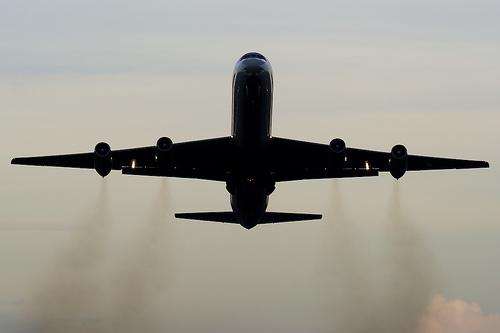
\includegraphics[width=0.48\columnwidth]{../images/test6} 
	} 
	\subfigure[分割图] { \label{fig:b4} 
		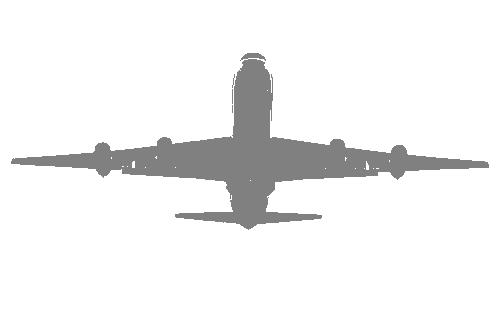
\includegraphics[width=0.48\columnwidth]{../result/test6seg} 
	} 
	\caption{使用Kmeans聚类算法进行图像分割} 
	\label{fig:4} 
\end{figure}

\begin{figure}[!h] \centering 
	\subfigure[原图像] { \label{fig:a2} 
		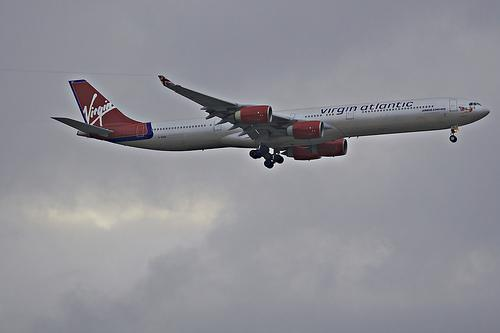
\includegraphics[width=0.48\columnwidth]{../images/test5} 
	} 
	\subfigure[分割图] { \label{fig:b2} 
		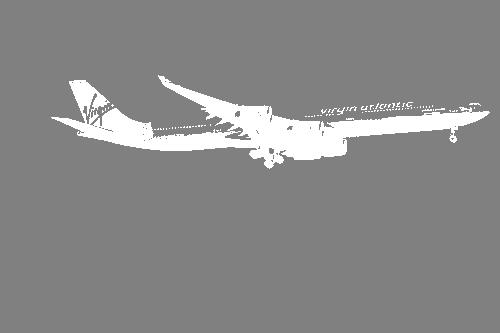
\includegraphics[width=0.48\columnwidth]{../result/test5seg} 
	} 
	\caption{使用Kmeans聚类算法进行图像分割} 
	\label{fig:1} 
\end{figure}

\begin{figure}[!h] \centering 
	\subfigure[原图像] { \label{fig:a3} 
		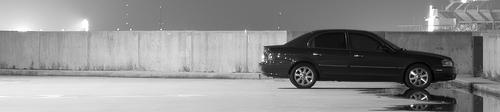
\includegraphics[width=0.48\columnwidth]{../images/test4} 
	} 
	\subfigure[分割图] { \label{fig:b3} 
		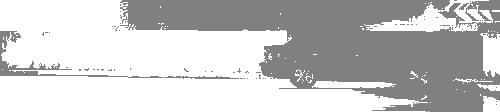
\includegraphics[width=0.48\columnwidth]{../result/test4seg} 
	} 
	\caption{使用Kmeans聚类算法进行图像分割} 
	\label{fig:2} 
\end{figure}

\begin{figure}[!h] \centering 
	\subfigure[原图像] { \label{fig:a} 
		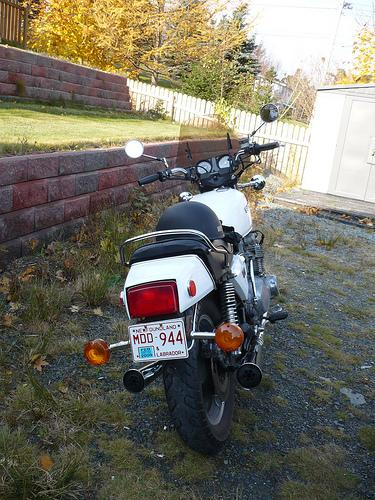
\includegraphics[width=0.48\columnwidth]{../images/test3} 
	} 
	\subfigure[分割图] { \label{fig:b} 
		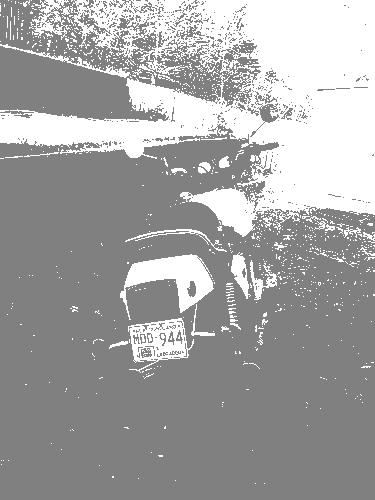
\includegraphics[width=0.48\columnwidth]{../result/test3seg} 
	} 
	\caption{使用Kmeans聚类算法进行图像分割} 
	\label{fig:3} 
\end{figure}



\begin{figure}[!h] \centering 
	\subfigure[原图像] { \label{fig:a5} 
		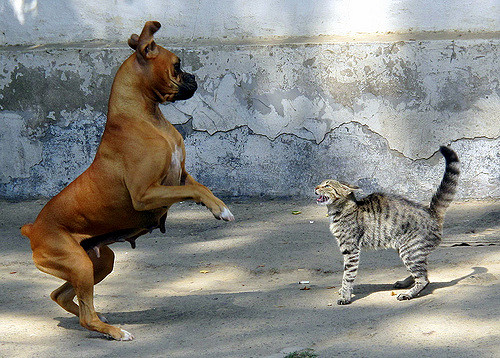
\includegraphics[width=0.48\columnwidth]{../images/test8} 
	} 
	\subfigure[分割图] { \label{fig:b5} 
		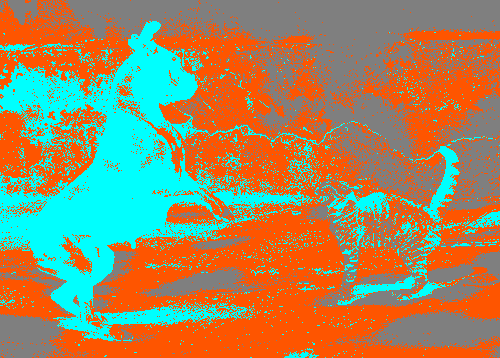
\includegraphics[width=0.48\columnwidth]{../result/test8seg.png} 
	} 
	\caption{使用Kmeans聚类算法进行图像分割} 
	\label{fig:5} 
\end{figure}

\begin{figure}[!h] \centering 
	\subfigure[原图像] { \label{fig:a6} 
		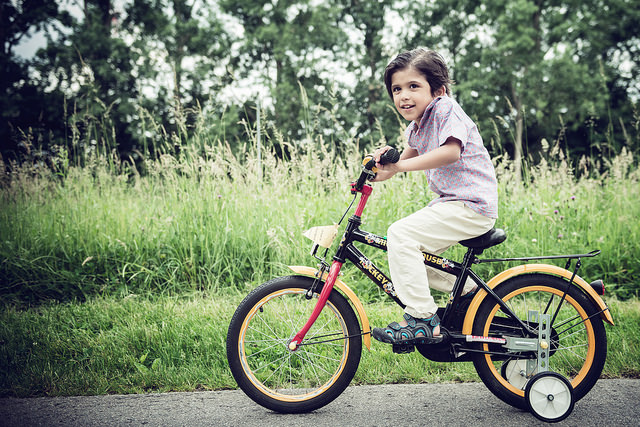
\includegraphics[width=0.48\columnwidth]{../images/test9} 
	} 
	\subfigure[分割图] { \label{fig:b6} 
		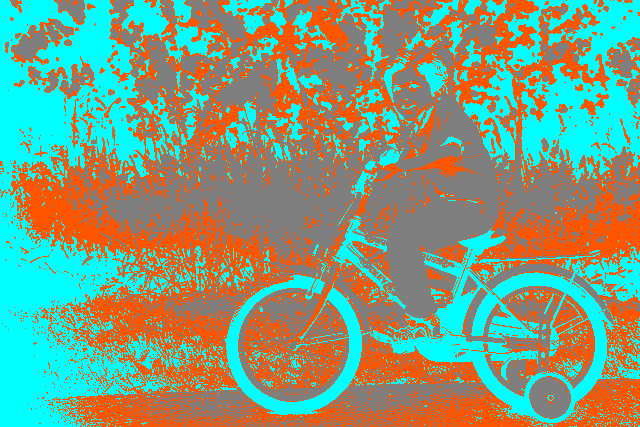
\includegraphics[width=0.48\columnwidth]{../result/test9seg.png} 
	} 
	\caption{使用Kmeans聚类算法进行图像分割} 
	\label{fig:6} 
\end{figure}

\begin{figure}[!h]
	\centering
	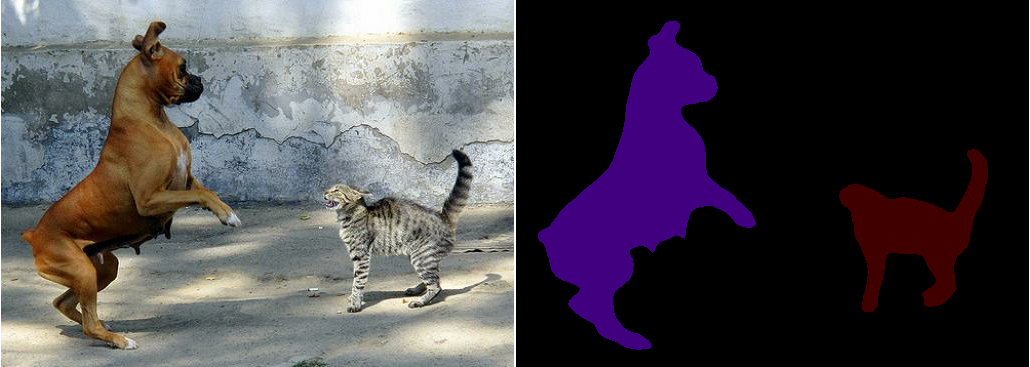
\includegraphics[width=0.96\columnwidth]{../result/test9deeplab}
	\caption{\label{fig:8}使用DeepLabV3算法进行图像分割}
\end{figure}

\begin{figure}[!h]
	\centering
	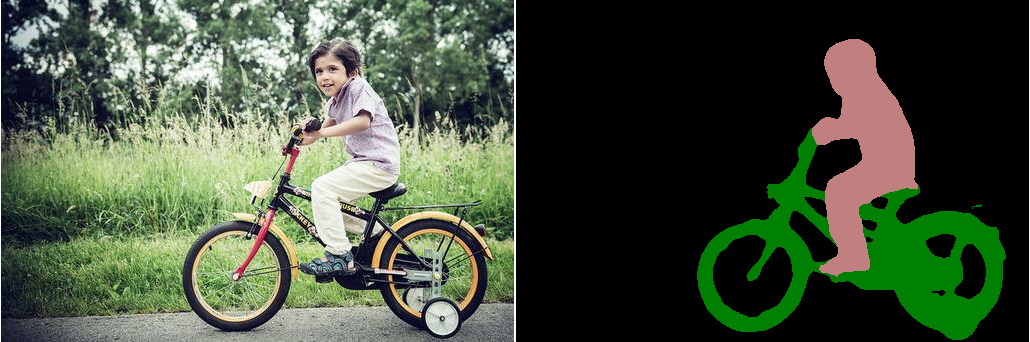
\includegraphics[width=0.96\columnwidth]{../result/test8deeplab}
	\caption{\label{fig:7}使用DeepLabV3算法进行图像分割}
\end{figure}

\end{document}